\chapter{CONDUCCIÓN PERMANENTE}

\section{Deducción de la ecuación general de la conducción}
Conducción es un mecanismo de transferencia de calor propio de los medios
solidos a nivel atómico.

\begin{figure}[!h]
\centering
\includegraphics[scale=1.00]{figura02_01.eps}
\caption{Conducción de calor en las tres dimensiones.}
\end{figure}

\begin{figure}[!h]
\centering
\includegraphics[scale=0.80]{figura02_02.eps}
\caption{Conducción de calor en una dirección.}
\end{figure}

\begin{equation*}
    \Delta x=\Delta y=\Delta z
\end{equation*}

\underline{Balance}:

\begin{equation}
    q_{xi}-q_{xs}+q_g=q_s
    \label{balance}
\end{equation}
Donde:
\begin{itemize}
    \item \emph{$q_{xi}$}: Calor que ingresa.
    \item \emph{$q_{xs}$}: Calor de sale.
    \item \emph{$q_g$}: Calor que se genera.
    \item \emph{$q_s$}: Calor sensible.
\end{itemize}

\begin{equation}
    q_{xi}=-k_x\,A_x\,\frac{\partial t}{\partial x}
    \label{qxi}
\end{equation}
\begin{equation}
    q_{xs}=q_{xi}+\frac{\partial q_{xi}}{\partial x}\,\Delta_x
    \label{qxs}
\end{equation}
\begin{equation}
    q_s=m\,C_p\,\frac{\partial t}{\partial\theta}
    \label{qs}
\end{equation}

Combinando las ecuaciones (\ref{qxi}), (\ref{qxs}), (\ref{qs}) en
(\ref{balance}):
\begin{equation*}
    q_{xi}-\left(q_{xi}+\frac{\partial q_{xi}}{\partial x}\,\Delta_x\right)+q_g
    =m\,C_p\,\frac{\partial t}{\partial\theta}
\end{equation*}
\begin{equation*}
    -\frac{\partial q_{xi}}{\partial x}\,\Delta_x+q_g
    =m\,C_p\,\frac{\partial t}{\partial\theta}
\end{equation*}
\begin{equation*}
    -\frac{\partial}{\partial x}
    \left(-k_x\,A_x\,\frac{\partial t}{\partial x}\right)\,\Delta_x+q_g
    =m\,C_p\,\frac{\partial t}{\partial\theta}
\end{equation*}
\begin{equation*}
    k_x\,A_x\,\frac{\partial^{2}t}{\partial x^2}\,\Delta_x+q_g
    =m\,C_p\,\frac{\partial t}{\partial\theta}
\end{equation*}

Considerando que:
\begin{equation*}
    A_x\,\Delta x=\Delta z\,\Delta y\,\Delta x=\Delta V
\end{equation*}

Por tanto:
\begin{equation*}
    k_x\,\Delta V\,\frac{\partial^{2}t}{\partial x^2}+q_g
    =m\,C_p\,\frac{\partial t}{\partial\theta}
\end{equation*}
\begin{equation}
    \frac{\partial^{2}t}{\partial x^2}+\frac{q_g}{k_x\,\Delta V}
    =\frac{m\,C_p}{k_x\,\Delta V}\,\frac{\partial t}{\partial\theta}
    \label{base1}
\end{equation}

Si consideramos que:
\begin{equation}
    \frac{q_g}{k_x\,\Delta V}=q'_g
    \label{qg}
\end{equation}
\begin{equation*}
    \rho=\frac{m}{\Delta V}
\end{equation*}
\begin{equation}
    \frac{m\,C_p}{k_x\,\Delta V}=\rho\frac{C_p}{k_x}=\frac{1}{\alpha}
    \label{difusividad}
\end{equation}

Donde:
\begin{itemize}
    \item \emph{$\alpha$}: Coeficiente de difusividad térmica.
\end{itemize}

\begin{equation}
    \alpha=\frac{k_x}{\rho\,C_p}
    \label{alpha}
\end{equation}

Combinando las ecuaciones (\ref{qg}) y (\ref{difusividad}) en (\ref{base1}):
\begin{equation}
    \frac{\partial^{2}t}{\partial x^2}+q'_g
    =\frac{1}{\alpha}\,\frac{\partial t}{\partial\theta}
    \label{base2}
\end{equation}

Y generalizando a las 3 dimensiones, se obtiene la \textbf{Ecuación general de
la conducción}:
\begin{equation}
    \frac{\partial^{2}t}{\partial x^2}
    +\frac{\partial^{2}t}{\partial y^2}
    +\frac{\partial^{2}t}{\partial z^2}+q'_g
    =\frac{1}{\alpha}\,\frac{\partial t}{\partial\theta}
    \label{base3}
\end{equation}

Valida para materiales isótropos, es decir:
\begin{equation*}
    k_x=k_y=k_z
\end{equation*}

\section{Casos particulares}

\subsection{Ecuación de \emph{Laplace}}
Para $q'_g=0$ y $\dfrac{\partial t}{\partial\theta}=0$, se tiene la ecuación
para conducción permanente:

\begin{equation}
    \frac{\partial^{2}t}{\partial x^2}
    +\frac{\partial^{2}t}{\partial y^2}
    +\frac{\partial^{2}t}{\partial z^2}=0
    \label{laplace}
\end{equation}

\subsection{Ecuación de \emph{Fourier}}
Para $q'_g=0$, se tiene la ecuación para conducción no permanente:

\begin{equation}
    \frac{\partial^{2}t}{\partial x^2}
    +\frac{\partial^{2}t}{\partial y^2}
    +\frac{\partial^{2}t}{\partial z^2}
    =\frac{1}{\alpha}\,\frac{\partial t}{\partial\theta}
    \label{fourier}
\end{equation}

\subsection{Ecuación de \emph{Poisson}}
Para $\dfrac{\partial t}{\partial\theta}=0$, se obtiene:

\begin{equation}
    \frac{\partial^{2}t}{\partial x^2}
    +\frac{\partial^{2}t}{\partial y^2}
    +\frac{\partial^{2}t}{\partial z^2}+q'_g=0
    \label{poisson}
\end{equation}

\section{Ecuación de \emph{Fourier} para conducción permanente}

\begin{figure}[!h]
\centering
\includegraphics[scale=1.20]{figura02_03.eps}
\caption{Conducción permanente lineal y no lineal.}
\end{figure}

\subsection{Caso: Distribución lineal}
\begin{equation*}
    q_x\propto A_x
\end{equation*}
\begin{equation*}
    q_x\propto\Delta t
\end{equation*}
\begin{equation*}
    q_x\propto \frac{1}{\Delta x}
\end{equation*}

\begin{equation*}
    q_x\propto \frac{A_x \Delta t}{\Delta x}
\end{equation*}

Ecuación de \emph{Fourier} para una distribución lineal:
\begin{equation}
    q_x=k\frac{A_x \Delta t}{\Delta x}
    \label{fourier}
\end{equation}

\subsection{Caso: Distribución no lineal}
\begin{equation*}
    \tan(\alpha)=\frac{\Delta t}{\Delta x}=\text{pendiente}
\end{equation*}

\begin{figure}[!h]
\centering
\includegraphics[scale=1.20]{figura02_04.eps}
\caption{Conducción permanente no lineal.}
\end{figure}

\begin{equation*}
    \frac{\Delta t}{\Delta x}=\frac{t_i-t_1}{x_1}
\end{equation*}
\begin{equation}
    t_1=t_i-x_1\frac{\Delta t}{\Delta x}
\end{equation}
\begin{equation*}
    \frac{\Delta t}{\Delta x}=\frac{t_1-t_2}{x_2}
\end{equation*}
\begin{equation}
    t_2=t_1-x_2\frac{\Delta t}{\Delta x}
\end{equation}

\section{Aplicación de la ecuación de \emph{Fourier} a varias geometrías de
cuerpo}

\subsection{Caso: Pared plana}
\begin{figure}[!h]
\centering
\includegraphics[scale=1.20]{figura02_05.eps}
\caption{Pared plana.}
\end{figure}

\begin{equation*}
    q_x
    =k_x\,A_x\,\frac{\Delta t}{\Delta x}
    =\frac{\Delta t}{\frac{\Delta x}{k_x\,A_x}}
    =\frac{\Delta t}{R}
\end{equation*}
\begin{equation*}
    R\,\text{(resistencia térmica)}=\frac{\Delta x}{k_x\,A_x}
\end{equation*}

\subsection{Caso: Paredes planas en serie}
\begin{figure}[!h]
\centering
\includegraphics[scale=1.20]{figura02_06.eps}
\caption{Paredes planas en serie.}
\end{figure}

La cantidad de calor que atraviesa cada pared es el mismo:
\begin{equation}
    q_x=q_{xa}=q_{xb}
\end{equation}

Por tanto:
\begin{equation}
    q_{xa}=\frac{t_i-t_{ab}}{R_a}
    \label{qxa}
\end{equation}
\begin{equation}
    q_{xb}=\frac{t_{ab}-t_o}{R_b}
    \label{qxb}
\end{equation}

Igualando las ecuaciones (\ref{qxa}) y (\ref{qxb}):
\begin{equation*}
    \frac{t_i-t_{ab}}{R_a}=\frac{t_{ab}-t_o}{R_b}
\end{equation*}
\begin{equation*}
    t_i-t_{ab}=\frac{R_a}{R_b}\,t_{ab}-t_o
\end{equation*}
\begin{equation*}
    t_i-t_{ab}=\frac{R_a}{R_b}\,t_{ab}-\frac{R_a}{R_b}\,t_o
\end{equation*}
\begin{equation*}
    \left(\frac{R_a}{R_b}+1\right)\,t_{ab}=t_i+\frac{R_a}{R_b}\,t_o
\end{equation*}
\begin{equation}
    t_{ab}=\dfrac{t_i+\frac{R_a}{R_b}\,t_0}{\frac{R_a}{R_b}+1}
    \label{tab}
\end{equation}

Combinando (\ref{qxa}) y (\ref{tab}):
\begin{equation*}
\begin{split}
    q_{xa}
        &=\dfrac{t_i-\frac{t_i+\frac{R_a}{R_b}\,t_o}{\frac{R_a}{R_b}+1}}{R_a}
         =\dfrac{t_i-\frac{\frac{R_b\,t_i+R_a\,t_o}{R_b}}{\frac{R_a+R_b}{R_b}}}
          {R_a}
         =\dfrac{t_i-\frac{R_b\,t_i+R_a\,t_o}{R_a+R_b}}{R_a}\\
        &=\dfrac{\frac{R_a\,t_i+R_b\,t_i-R_b\,t_i-R_a\,t_o}{R_a+R_b}}{R_a}
         =\dfrac{\frac{R_a\,t_i-R_a\,t_o}{R_a+R_b}}{R_a}
         =\dfrac{\frac{R_a\,(t_i-t_o)}{R_a+R_b}}{R_a}\\
        &=\frac{t_i-t_o}{R_a+R_b}\\
\end{split}
\end{equation*}

Generalizando para $n$ materiales:
\begin{equation}
    q_x=\frac{t_i-t_o}{\sum R}
\end{equation}

Por analogía eléctrica:
\begin{figure}[!h]
\centering
\includegraphics[scale=1.00]{figura02_07.eps}
\caption{Analogía eléctrica.}
\end{figure}

\begin{equation*}
    I=I_a+I_b
\end{equation*}

\begin{equation*}
\def\arraystretch{1.4}
\begin{array}{@{}cll@{}}
I=\dfrac{\Delta V}{\sum R} & \rightarrow & q=\dfrac{\Delta T}{\sum R} \\
\end{array}
\end{equation*}

\subsection{Caso: Pared plana compuesta}
\begin{figure}[!h]
\centering
\includegraphics[scale=1.20]{figura02_08.eps}
\caption{Pared plana compuesta.}
\end{figure}

\begin{figure}[!h]
\centering
\includegraphics[scale=1.20]{figura02_09.eps}
\caption{Analogía eléctrica.}
\end{figure}

\begin{equation*}
    q=\frac{t_i-t'}{R_a}\,\rightarrow\,t'=t_i-q\,R_a
\end{equation*}
\begin{equation*}
    q=\frac{t_i-t''}{R_a+R_{eq}}\,\rightarrow\,t''=t_i-q\,(R_a+R_{eq})
\end{equation*}
\begin{equation*}
    q=\frac{t'''-t_o}{R_g}\,\rightarrow\,t'''=q\,R_g+t_o
\end{equation*}

\subsection{Caso: Conducto cilíndrico}
\begin{figure}[!h]
\centering
\includegraphics[scale=1.10]{figura02_10.eps}
\caption{Cilindro hueco.}
\end{figure}

Para hallar la resistencia termina, existen dos posibles áreas a usar:

\begin{enumerate}
\item Área promedio, que es una aproximación:
\begin{equation*}
    A=\frac{A_i+A_e}{2}
\end{equation*}
\item Área logarítmica, que es un calculo exacto; que se deduce de la siguiente
manera:
\begin{equation*}
    A(\text{cilindro})=2\pi\,r\,L
\end{equation*}

Utilizando la ecuación de \emph{Fourier} (\ref{fourier}):
\begin{equation*}
    q=-k\,A\,\frac{dt}{dr}
\end{equation*}
\begin{equation*}
    \frac{dr}{A}=-\frac{k}{q}\,dt
\end{equation*}
\begin{equation*}
    \frac{dr}{2\pi\,r\,L}=-\frac{k}{q}\,dt
\end{equation*}
\begin{equation*}
    \int_{r_i}^{r_e}\frac{dr}{r}=\int_{t_o}^{t_i}-\frac{2\pi\,L\,k}{q}\,dt
\end{equation*}
\begin{equation*}
    \ln\left(\frac{r_e}{r_i}\right)=-\frac{2\pi\,L\,k}{q}(t_i-t_o)
\end{equation*}
\begin{equation*}
    \Delta t=t_o-t_i
\end{equation*}
\begin{equation*}
    \ln\left(\frac{r_e}{r_i}\right)=\frac{2\pi\,L\,k}{q}\Delta t
\end{equation*}
\begin{equation}
    q=\frac{2\pi\,L\,k\,\Delta t}{\ln\left(\frac{r_e}{r_i}\right)}
    \label{cilindro1}
\end{equation}

Comparando (\ref{fourier}) con (\ref{cilindro1}):
\begin{equation*}
    \frac{A}{\Delta r}=\frac{2\pi\,L}{\ln\left(\frac{r_e}{r_i}\right)}
\end{equation*}
\begin{equation*}
    A=\frac{2\pi\,L\,\Delta r}{\ln\left(\frac{r_e}{r_i}\right)}
\end{equation*}
\begin{equation*}
    A=\frac{2\pi\,L\,(r_e-r_i)}{\ln\left(\frac{r_e}{r_i}\right)}
\end{equation*}
\begin{equation*}
    A=\frac{2\pi\,L\,r_e-2\pi\,L\,r_i}
    {\ln\left(\frac{2\pi\,L\,r_e}{2\pi\,L\,r_i}\right)}
\end{equation*}
\begin{equation}
    A=\frac{A_e-A_i}{\ln\left(\frac{A_e}{A_i}\right)}
    \label{cilindro2}
\end{equation}
\end{enumerate}

\subsection{Caso: Superficies cilíndricas en serie}
\begin{figure}[!h]
\centering
\includegraphics[scale=1.10]{figura02_11.eps}
\caption{Cilindros en serie.}
\end{figure}

\begin{figure}[!h]
\centering
\includegraphics[scale=1.10]{figura02_12.eps}
\caption{Analogía eléctrica.}
\end{figure}

\begin{equation*}
    q=\frac{t_i-t_o}{R_1+R_2+R_3}
\end{equation*}
\begin{equation*}
    q=\frac{t_i-t_o}{\sum R}
\end{equation*}

\subsection{Caso: Superficies cilíndricas compuestas}
\begin{figure}[!h]
\centering
\includegraphics[scale=1.10]{figura02_13.eps}
\caption{Cilindros compuestos.}
\end{figure}

\begin{figure}[!h]
\centering
\includegraphics[scale=1.10]{figura02_14.eps}
\caption{Analogía eléctrica.}
\end{figure}

\subsection{Caso: Esferas huecas}
\begin{figure}[!h]
\centering
\includegraphics[scale=1.10]{figura02_15.eps}
\caption{Esfera hueca.}
\end{figure}

\begin{equation*}
    A(\text{esfera})=4\pi\,r^2
\end{equation*}

Utilizando la ecuación de \emph{Fourier} (\ref{fourier}):
\begin{equation*}
    q=-k\,A\,\frac{dt}{dr}
\end{equation*}
\begin{equation*}
    \frac{dr}{A}=-\frac{k}{q}\,dt
\end{equation*}
\begin{equation*}
    \frac{dr}{4\pi\,r^2}=-\frac{k}{q}\,dt
\end{equation*}
\begin{equation*}
    \int_{r_i}^{r_e}\frac{dr}{r^2}=\int_{t_o}^{t_i}-\frac{4\pi\,k}{q}\,dt
\end{equation*}
\begin{equation*}
    \frac{1}{r_i}-\frac{1}{r_e}=-\frac{4\pi\,k}{q}(t_i-t_o)
\end{equation*}
\begin{equation*}
    \Delta t=t_o-t_i
\end{equation*}
\begin{equation*}
    \frac{1}{r_i}-\frac{1}{r_e}=\frac{4\pi\,k}{q}\Delta t
\end{equation*}
\begin{equation}
    q=\frac{4\pi\,k\,\Delta t}{\frac{1}{r_i}-\frac{1}{r_e}}
    \label{esfera1}
\end{equation}

Comparando (\ref{fourier}) con (\ref{esfera1}):
\begin{equation*}
    \frac{A}{\Delta r}=\frac{4\pi}{\frac{1}{r_i}-\frac{1}{r_e}}
\end{equation*}
\begin{equation*}
    A=\frac{4\pi\,\Delta r}{\frac{1}{r_i}-\frac{1}{r_e}}
\end{equation*}
\begin{equation*}
    A=\frac{4\pi\,\Delta r}{\frac{r_e-r_i}{r_i\,r_e}}
\end{equation*}
\begin{equation*}
    A=\frac{4\pi\,\Delta r}{\frac{\Delta r}{r_i\,r_e}}
\end{equation*}
\begin{equation*}
    A=4\pi\,r_i\,r_e
\end{equation*}
\begin{equation}
    A=\sqrt{A_i\,A_e}
    \label{esfera2}
\end{equation}

\subsubsection{Calculo del espesor óptimo-económico de un aislante}
Coeficiente $k$:

\begin{itemize}
    \item Materiales conductores: $k\propto 1/T$.\\
        \underline{Ejemplo}: Acero al cromo (10\% Cr).
        \begin{equation*}
        \def\arraystretch{1.3}
        \begin{array}{@{}cl@{}}
        \toprule
        t=20^\circ\text{C} & k=27[\text{kcal}/\text{mh}^\circ\text{C}]\\
        \cmidrule(l){1-2}
        t=400^\circ\text{C} & k=25[\text{kcal}/\text{mh}^\circ\text{C}]\\
        \bottomrule
        \end{array}
        \end{equation*}
    \item Materiales no conductores: $k\propto T$.\\
        \underline{Ejemplo}: Amianto.
        \begin{equation*}
        \def\arraystretch{1.3}
        \begin{array}{@{}cl@{}}
        \toprule
        t=0^\circ\text{C} & k=0.134[\text{kcal}/\text{mh}^\circ\text{C}]\\
        \cmidrule(l){1-2}
        t=100^\circ\text{C} & k=0.165[\text{kcal}/\text{mh}^\circ\text{C}]\\
        \bottomrule
        \end{array}
        \end{equation*}
\end{itemize}

El costo del espesor se basa en el costo total:
\begin{equation}
    C_{\text{total}}=C_{\text{fijo}}+C_{\text{variable}}
\end{equation}

El \textbf{costo fijo} se basa en el gasto en material aislante:
\begin{equation*}
    C_{\text{fijo}}=A_T [\text{m}^2]
\end{equation*}
\begin{equation*}
    A_T=A_1+A_2+A_3+\cdots+A_n=\sum_{i=1}^n A_i
\end{equation*}

Se puede hacer cierta simplificación en los cálculos:
\begin{equation*}
    A_1\approx A_2\approx A_3\approx\cdots\approx A_n
\end{equation*}
\begin{equation*}
    A_T=nA_i
\end{equation*}

Por tanto:
\begin{equation*}
    C_{\text{fijo}}=nA_i[\text{m}^2]
    CA\left[\frac{\text{Bs}}{\text{m}^2}\right]
    \frac{1}{TV[\text{año}]}
\end{equation*}

Donde:
\begin{itemize}
    \item $CA$: Costo del aislante.
    \item $TV$: Tiempo de vida.
\end{itemize}

El \textbf{costo variable} se basa en el gasto de la generación de calor:
\begin{figure}[!h]
\centering
\includegraphics[scale=1.10]{figura02_16.eps}
\end{figure}

\begin{equation*}
    q=\frac{t_i-t_o}{R_p+R_1+R_2+\cdots+R_n}
\end{equation*}
\begin{equation*}
    R_T=R_1+R_2+R_3+\cdots+R_n=\sum_{i=1}^n R_i
\end{equation*}
\begin{equation*}
    q=\frac{t_i-t_o}{R_p+\sum_{i=1}^n R_i}
\end{equation*}

Se puede hacer cierta simplificación en los cálculos:
\begin{equation*}
    R_1\approx R_2\approx R_3\approx\cdots\approx R_n
\end{equation*}
\begin{equation*}
    R_T=nR_i
\end{equation*}
\begin{equation*}
    q=\frac{t_i-t_o}{R_p+nR_i}
\end{equation*}

Por tanto:
\begin{equation*}
    C_{\text{variable}}=\frac{t_i-t_o}{R_p+nR_i}
    \left[\frac{\text{kcal}}{\text{h}}\right]
    \frac{1[\text{kg}]}{PC[\text{kcal}]}
    CC\left[\frac{\text{Bs}}{\text{kg}}\right]
    FU\left[\frac{\text{h}}{\text{año}}\right]
\end{equation*}

Donde:
\begin{itemize}
    \item $PC$: Poder calorífico.
        \begin{enumerate}
            \item Combustible solido ($kcal/kg$).
            \item Combustible liquido ($kcal/lt$).
            \item Combustible gaseoso ($kcal/m^3$).
        \end{enumerate}
    \item $CC$: Costo de combustible.
        \begin{enumerate}
            \item Combustible solido ($Bs/kg$).
            \item Combustible liquido ($Bs/lt$).
            \item Combustible gaseoso ($Bs/m^3$).
        \end{enumerate}
    \item $FU$: Frecuencia de uso.
        \begin{enumerate}
            \item Horas de uso al día ($\text{hr}/\text{día}$).
            \item Días de uso al mes ($\text{día}/\text{mes}$).
            \item Meses de uso al año ($\text{mes}/\text{año}$).
        \end{enumerate}
\end{itemize}

\begin{equation}
    C_{\text{total}}=C_{\text{fijo}}+C_{\text{variable}}=nA+\frac{B}{R_p+nR_i}
\end{equation}

Por tanto:
\begin{equation*}
    C_{\text{fijo}}\propto n
\end{equation*}
\begin{equation*}
    C_{\text{variable}}\propto 1/n
\end{equation*}

Para el calculo del número de capas de aislante se pueden usar dos métodos:
\begin{itemize}
    \item Gráfico: Realizando los trazados del costo fijo y costo variable,
    puede hallarse la gráfica de costo total, y calcular el valor mínimo.
        \begin{figure}[!h]
        \centering
        \includegraphics[scale=1.50]{figura02_17.eps}
        \end{figure}
    \item Analítico: Se calcula el valor mínimo de la función $C_T$ a través de
    su derivada:
        \begin{equation*}
            \frac{dC_T}{dn}=0
        \end{equation*}
\end{itemize}

\subsection{Caso: $k=\phi(t)$}
En tablas pueden encontrarse diferentes valores del coeficiente de conducción
según la temperatura.
\begin{equation*}
\def\arraystretch{1.5}
\begin{array}{@{}clll@{}}
\toprule
\text{Material} & t_1 & t_2 & t_3 \\
\cmidrule(l){1-4}
m_1 & k_1 & k_2 & k_3\\
\bottomrule
\end{array}
\end{equation*}

Para los valores intermedios puede realizarse una interpolación entre los
valores mas próximos.

\begin{figure}[!h]
\centering
\includegraphics[scale=1.00]{figura02_18.eps}
\end{figure}

Pueden usarse dos métodos:

\begin{enumerate}
    \item Calcular los coeficientes para la temperatura de entrada ($t_i$) y
        salida ($t_o$), y utilizar el promedio de ambas:
        \begin{equation*}
            t_i\rightarrow k_i
        \end{equation*}
        \begin{equation*}
            t_o\rightarrow k_o
        \end{equation*}
        \begin{equation*}
            \bar{k}=\frac{k_i+k_o}{2}
        \end{equation*}

    \item Calcular el promedio entre las temperaturas y calcular el coeficiente
        para esa temperatura por interpolación:
        \begin{equation*}
            \bar{t}=\frac{t_i+t_o}{2}
        \end{equation*}
        \begin{equation*}
            \bar{t}\rightarrow \bar{k}
        \end{equation*}
\end{enumerate}

\section{Conduccióń permanente bidireccional}
Existen varios métodos de solución:

\begin{itemize}
    \item Método analítico o método numérico.
    \item Método por analogía o método de mapas.
    \item Método empírico.
\end{itemize}

\subsection{Método numérico}

\underline{Pasos:}
\begin{itemize}
    \item Dibujar la sección.
        \begin{figure}[!h]
        \centering
        \includegraphics[scale=0.80]{figura02_19.eps}
        \end{figure}
    \item Dibujar una malla cuadrada tal que $\Delta x=\Delta y$.
        \begin{figure}[!h]
        \centering
        \includegraphics[scale=1.60]{figura02_20.eps}
        \end{figure}
    \item Identificar los nodos de la malla.
        \begin{figure}[!h]
        \centering
        \includegraphics[scale=2.40]{figura02_21.eps}
        \end{figure}
    \item Obtener ecuaciones lineales para cada nodo interno, basado en la
        expresión matemática del método numérico.
        \begin{figure}[!h]
        \centering
        \includegraphics[scale=2.40]{figura02_22.eps}
        \end{figure}

        \underline{Balance de calor en el nodo $0$}:
        \begin{equation*}
            \text{calor que ingresa a 0}=\text{energía que queda en 0}
        \end{equation*}
        \begin{equation*}
            q_{10}+q_{20}+q_{30}+q_{40}+q_{50}=q_0
        \end{equation*}
        Se considera al nodo $0$ un sumidero de calor, por tanto $q_0=0$.
        \begin{equation*}
            k_x A_x\frac{t_1-t_0}{\Delta x}+
            k_y A_y\frac{t_2-t_0}{\Delta y}+
            k_x A_x\frac{t_3-t_0}{\Delta x}+
            k_y A_y\frac{t_4-t_0}{\Delta y}=0
        \end{equation*}
        \begin{equation*}
            A_x=A_y
        \end{equation*}
        \begin{equation*}
            \Delta x=\Delta y
        \end{equation*}
        \begin{equation*}
            k_x=k_y
        \end{equation*}
        \begin{equation*}
            t_1-t_0+t_2-t_0+t_3-t_0+t_4-t_0=0
        \end{equation*}
        \begin{equation*}
            4t_0=t_1+t_2+t_3+t_4
        \end{equation*}
        \begin{equation*}
            t_0=\frac{t_1+t_2+t_3+t_4}{4}
        \end{equation*}
    \item Resolver el sistema de ecuaciones.
\end{itemize}

\subsection{Método de mapas de dos dimensiones}
\textbf{Mapa}: Es una representación gráfica de un objeto en un plano o en el
espacio.

\begin{figure}[!h]
\centering
\includegraphics[scale=1.60]{figura02_23.eps}
\end{figure}

\subsubsection{Deducción de la expresión de calor transmitido}
Sea: $q_1$ el calor transmitido a través de un cuadrado curvilíneo.
\begin{equation*}
    q_1=k_x A_x\frac{(t_i-t_o)}{\Delta x}
\end{equation*}

Sea: $q_s$ el calor transmitido por una senda de calor y $N_{cs}$ el número de
cuadrados curvilíneos en la senda de calor.
\begin{equation*}
    q_s=\frac{k_x A_x}{\Delta x}\left(\frac{t_i-t_o}{N_{cs}}\right)
\end{equation*}

Sea: $N_{s}$  el número de sendas en la sección.
\begin{equation*}
    q=N_s\frac{k_x A_x}{\Delta x}\left(\frac{t_i-t_o}{N_{cs}}\right)
\end{equation*}

Sabiendo que $A_x=\Delta y L$:
\begin{equation*}
    q=N_s\frac{k_x \Delta y L}{\Delta x}\left(\frac{t_i-t_o}{N_{cs}}\right)
\end{equation*}

Considerando que $\Delta x=\Delta y$:
\begin{equation*}
    q=N_s k_x L\left(\frac{t_i-t_o}{N_{cs}}\right)
\end{equation*}
\begin{equation}
    \frac{q}{L}=\frac{N_s}{N_{cs}}\,k_x(t_i-t_o)
\end{equation}

Donde: $N_s/N_{cs}$ es la razón geométrica.

\subsection{Método aproximado}
La combinación del método numérico y el método de mapas nos da una método
exacto.

